%------------------------------------------------------------------------------
% Template file for the submission of papers to IUCr journals in LaTeX2e
% using the iucr document class
% Copyright 1999-2013 International Union of Crystallography
% Version 1.6 (28 March 2013)
%------------------------------------------------------------------------------

\documentclass[preprint]{iucr}              % DO NOT DELETE THIS LINE
\usepackage{verbatim}
     %-------------------------------------------------------------------------
     % Information about journal to which submitted
     %-------------------------------------------------------------------------
     \journalcode{A}              % Indicate the journal to which submitted
                                  %   A - Acta Crystallographica Section A
                                  %   B - Acta Crystallographica Section B
                                  %   C - Acta Crystallographica Section C
                                  %   D - Acta Crystallographica Section D
                                  %   E - Acta Crystallographica Section E
                                  %   F - Acta Crystallographica Section F
                                  %   J - Journal of Applied Crystallography
                                  %   M - IUCrJ
                                  %   S - Journal of Synchrotron Radiation

\usepackage{amsmath}

\begin{document}                  % DO NOT DELETE THIS LINE

     %-------------------------------------------------------------------------
     % The introductory (header) part of the paper
     %-------------------------------------------------------------------------

     % The title of the paper. Use \shorttitle to indicate an abbreviated title
     % for use in running heads (you will need to uncomment it).

\title{The Expand-Maximize-Compress Single Particle Imaging Algorithm}
%\shorttitle{Short Title}

     % Authors' names and addresses. Use \cauthor for the main (contact) author.
     % Use \author for all other authors. Use \aff for authors' affiliations.
     % Use lower-case letters in square brackets to link authors to their
     % affiliations; if there is only one affiliation address, remove the [a].

\cauthor[a]{Kartik}{Ayyer}{kartik.ayyer@desy.de}
\author[b]{Ti-Yen}{Lan}
\author[c]{N. Duane}{Loh}
\author[b]{Veit}{Elser}

\aff[a]{Center for Free-Electron Laser Science, Deutsches Elektronen-Synchrotron DESY, Notkestra{\ss}e 85, 22607 Hamburg, \country{Germany}}
\aff[b]{Second affiliation address}
\aff[c]{Centre for Bio-imaging Sciences, National University of Singapore, Singapore 117543.}

     % Use \shortauthor to indicate an abbreviated author list for use in
     % running heads (you will need to uncomment it).

%\shortauthor{Soape, Author and Doe}

     % Use \vita if required to give biographical details (for authors of
     % invited review papers only). Uncomment it.

%\vita{Author's biography}

     % Keywords (required for Journal of Synchrotron Radiation only)
     % Use the \keyword macro for each word or phrase, e.g. 
     % \keyword{X-ray diffraction}\keyword{muscle}

%\keyword{keyword}

     % PDB and NDB reference codes for structures referenced in the article and
     % deposited with the Protein Data Bank and Nucleic Acids Database (Acta
     % Crystallographica Section D). Repeat for each separate structure e.g
     % \PDBref[dethiobiotin synthetase]{1byi} \NDBref[d(G$_4$CGC$_4$)]{ad0002}

%\PDBref[optional name]{refcode}
%\NDBref[optional name]{refcode}

\maketitle                        % DO NOT DELETE THIS LINE

\begin{synopsis}
Supply a synopsis of the paper for inclusion in the Table of Contents.
\end{synopsis}

\begin{abstract}
Abstract goes here.
\end{abstract}


     %-------------------------------------------------------------------------
     % The main body of the paper
     %-------------------------------------------------------------------------
     % Now enter the text of the document in multiple \section's, \subsection's
     % and \subsubsection's as required.

\section{Introduction}

\subsection{Purpose software package}
 A Computer Program article should make clear the novelty of the program and its scientific context. 

\section{Structure of package}
This software package uses the EMC algorithm to reconstruct a 3D diffraction volume from noisy, randomly-oriented single particle diffraction patterns. These patterns could be from simulations or actual single-particle experiments, where the minimum input are: a configuration file, a file with detector coordinates and pixel status, and a sparse representation of the photon data from diffraction patterns \figref{flowchart}. Here?s an example of the configuration file that simulates a single-particle imaging data stream and reconstructs the 3D intensities afterwards:


\subsection{Typical experiment and key parameters}

\subsection{Data stream simulator}

\subsection{EMC algorithm}

\subsection{Convenience utilities}
\label{subsec:conv}
Here, the EMC algorithm is implemented with hybrid openMPI+openMP, and hence suitable for shared and/or distributed memory systems. 

Several convenience utilities are included to help prepare the data for or view the results from the EMC reconstruction algorithm. These utilities are briefly described here. 

\begin{enumerate}
\item{\bf init\_new\_recon.py.} This Python utility compiles the C executables in the package, and makes them plus other the rest of the utilities available in a newly initialized reconstruction sub-directory.
\item{\bf sim\_setup.py.} This Python utility simulates a single-particle data stream using the parameters listed in the configuration file. This utility, in turn, calls the following utilities that all depend on the configuration file.
\item{\bf make\_densities.py.} Creates an electron density map from a PDB file, given the resolution and field of view expected from the configuration file.
\item{\bf make\_intensities.py}. Creates a set of 3D diffraction intensities from an electron density map and the experimental parameters found in the configuration file.  
\item{\bf make\_data.py}. Simulates a sparse photon diffraction pattern using a 3D diffraction volume (e.g. the one generated by make_intensities.py), and the configuration file.
\item{\bf make\_quaternions.py}. Creates a list of quasi-uniform rotation group samples based on a refinement scheme of the 600-cell.
\item{\bf make\_powder.py}. Makes a virtual powder pattern from the sparse photon format adopted in this package.
\item{\bf run\_emc.py}. Starts the EMC reconstruction by calling its MPI+openMP implementation in C. Includes a few convenience operations like increasing the sampling of the rotation group.
\item{\bf autoplot.py}. Renders the results of the EMC reconstruction with the option of automatically updating the plots when newer intensities become available.
\end{enumerate}

\subsection{Data formats}
\subsubsection{Configuration file}
The configuration file is used to pass parameters and file names to the main reconstruction code as well as to the various utilities. The file has the standard \texttt{key = value} format with the parameters for different modules grouped by module names in square brackets. There is a global \texttt{[parameters]} module containing information about the experimental setup. A typical configuration file is shown in Fig.~\ref{fig:config}. This default file also shows the use of special keywords used to point to other configuration file parameters (eg. \texttt{in\_photons\_file}). The \texttt{[parameters]} module is described below. For other modules, refer to the relevant convenience utility in Section~\ref{subsec:conv}.

The basic parameters of the experiment are:
\begin{itemize}
\item \texttt{detd}: Detector distance in mm
\item \texttt{lambda}: Wavelength in \AA
\item \texttt{detsize}: Detector size (assuming square detector) in pixels
\item \texttt{pixsize}: Pixel size in mm
\item \texttt{stoprad}: Radius of beamstop in pixels
\item \texttt{polarization}: Polarization direction (can be x, y, or none)
\end{itemize}

\subsubsection{Detector file}
The detector file is an ASCII (human readable) file which describes various properties of the detector. The first line of the file contains a single number which represents the number of pixels. Following that, for each pixel, there are five columns of numbers. The first three columns give the 3D coordinates of the detector pixel in voxels, where the voxels refer to the 3D grid containing the intensity model. The next column gives the product of the polarization and solid angle corrections for that pixel. The last column is an 8-byte unsigned integer whose value is used by the EMC code as well as other utilities to categorize the pixel. Currently, there are three categories:
\begin{itemize}
\item 0: Good pixel, used to determine the orientation of a given frame.
\item 1: These pixels will not be used to determine the orientation, but will still be merged into the 3D grid using the orientations calculated from category 0 pixels.
\item 2: Bad pixel. Pixels whose value will be used neither to determine the orientation nor to calculate the merged 3D intensities.
\end{itemize}

\subsubsection{Photons file (emc format)}
Since the data in many relevant experiments utilizing the EMC algorithm have very few photons/frame, a sparse binary format is used to store the data. Instead of storing the number of counts at each pixel, only the locations of non-zero counts are stored. since most of the non-zero counts are ones, only the locations of those are stored. For the rest, two numbers are stored, the location and photon count. 

The header resides in the first 1024 bytes. The first 4 bytes are a 32 bit integer giving the number of data frames (\texttt{num\_data}) contained in the file. The next 4 bytes are also a 32 bit integer giving the number of pixels in the detector file used to number the pixels. The next 1016 bytes are currently empty (filled with zeros).

After this, there are \texttt{num\_data} 32 bit integers giving the number of one-photon events in each frame (\texttt{ones}). Similarily, there are \texttt{num\_data} integers giving the number of multi-photon events (\texttt{multi}). Let the sum of all numbers in the \texttt{ones} and \texttt{multi} arrays be \texttt{total\_ones} and \texttt{total\_multi}. 
\appendix
\section{Solid angle correction for square detectors}
Calculation of solid angle 

\section{Frame-by-frame intensity scale factor updates}
In many real world applications, the incident fluence on each particle will be different. The default implementation in \citeasnoun{loh2009} assumes uniform incident fluence. Here we derive the likelihood maximizing update rule employed in this package when the \texttt{need\_scaling} option is turned on. The approach used is similar to that employed in \citeasnoun{loh2010}, except for a Poisson probability model rather than Gaussian.
Let $d$, $r$ and $t$ represent the indices for the frame number, the orientation number and the pixel number respectively. The number of photons in frame $d$ at pixel $t$ is given by $K_{dt}$, and the value of the intensity in the tomogram with orientation $r$ at pixel $t$ is $W_{rt}$. In addition, one assumes a scale factor $\phi_d$ which is proportional to the incident fluence on the particle in frame $d$. Thus, 
\begin{align}
P_{dr} &= \frac{R_{dr}}{\sum\limits_r R_{dr}} \\
\mathrm{with, }\;R_{dr} &= \prod_t \frac{(W_{rt}\phi_d)^{K_{dt}} e^{-W_{rt}\phi_d}}{K_{dt}!}
\end{align}
is the probability of frame $d$ belonging to orientation $r$. In expectation maximization, one would like to find updates for the intensity tomograms, $W'$ and $\phi'$ which maximize the total log-likelihood $Q$ given by
\[Q(W', \phi') = \sum_d \sum_r \sum_t P_{dr} \left[K_{dt}\log(W'_{rt} \phi'_d) - W'_{rt} \phi'_d\right]\]
Here, $P_{dr}$ are the probabilities calculated using the current models for $W$ and $\phi$. Unfortunately, an analytical update rule for these quantities which maximizes $Q$ is not available. We use the strategy of updating one while keeping the other constant. Setting partial derivatives with respect to $W'$ and $\phi'$ equal to 0, we obtain
\begin{align}
W'_{rt} &= \frac{\sum\limits_d P_{dr} K_{dt}}{\sum\limits_d P_{dr} \phi_d} \\
\phi'_d &= \frac{\sum\limits_t K_{dt}}{\sum\limits_{rt} P_{dr} W_{rt}}
\end{align}

     %-------------------------------------------------------------------------
     % The back matter of the paper - acknowledgements and references
     %-------------------------------------------------------------------------

     % Acknowledgements come after the appendices

\ack{Acknowledgements}
N.D.L. would like to thank the support of the Lee Kuan Yew Endowment fund, and the assistance by the IT facility at the Centre for Bio-Imaging Sciences.

\referencelist[EMC]

%\begin{references}
%\reference{Author, A. \& Author, B. (1984). \emph{Journal} \textbf{Vol}, first page--last page.}
%\end{references}

     %-------------------------------------------------------------------------
     % TABLES AND FIGURES SHOULD BE INSERTED AFTER THE MAIN BODY OF THE TEXT
     %-------------------------------------------------------------------------

     % Simple tables should use the tabular environment according to this
     % model

\begin{table}
\caption{Caption to table}
\begin{tabular}{llcr}      % Alignment for each cell: l=left, c=center, r=right
 HEADING    & FOR        & EACH       & COLUMN     \\
\hline
 entry      & entry      & entry      & entry      \\
 entry      & entry      & entry      & entry      \\
 entry      & entry      & entry      & entry      \\
\end{tabular}
\end{table}

     % Postscript figures can be included with multiple figure blocks

\begin{figure}
\caption{Caption describing figure.}
\includegraphics{fig1.ps}
\end{figure}


\end{document}                    % DO NOT DELETE THIS LINE
%%%%%%%%%%%%%%%%%%%%%%%%%%%%%%%%%%%%%%%%%%%%%%%%%%%%%%%%%%%%%%%%%%%%%%%%%%%%%%
